\documentclass[10pt]{article}
\usepackage[margin=1in]{geometry}
\usepackage[T1]{fontenc}
\usepackage{lmodern}
\usepackage{amsmath,amssymb}
\usepackage{graphicx}
\usepackage{booktabs}
\usepackage[numbers,sort]{natbib}
\usepackage[hidelinks]{hyperref}
\usepackage{xcolor}
\renewcommand{\topfraction}{0.9}\renewcommand{\textfraction}{0.1}\renewcommand{\floatpagefraction}{0.8}
% generated by rewardshapes.analysis - do not edit
\newcommand{\nstarprefssparse}{3}
\newcommand{\nstarprefsdense}{3}
\newcommand{\nstarprefsshaped}{10}
\newcommand{\nstarprefsmulti}{3}
\newcommand{\nstarprefslava}{10}
\newcommand{\nstardemossparse}{1}
\newcommand{\nstardemosdense}{30}
\newcommand{\nstardemosshaped}{100}
\newcommand{\nstardemosmulti}{3}
\newcommand{\nstardemoslava}{3}
\newcommand{\epicprefssparse}{0.31}
\newcommand{\regretprefssparse}{0.001}
\newcommand{\epicprefsdense}{0.25}
\newcommand{\regretprefsdense}{0.014}
\newcommand{\epicprefsshaped}{0.58}
\newcommand{\regretprefsshaped}{0.041}
\newcommand{\epicprefsmulti}{0.27}
\newcommand{\regretprefsmulti}{0.001}
\newcommand{\epicprefslava}{0.28}
\newcommand{\regretprefslava}{0.003}
\newcommand{\epicdemossparse}{0.17}
\newcommand{\regretdemossparse}{0.001}
\newcommand{\epicdemosdense}{0.18}
\newcommand{\regretdemosdense}{0.001}
\newcommand{\epicdemosshaped}{0.67}
\newcommand{\regretdemosshaped}{0.002}
\newcommand{\epicdemosmulti}{0.19}
\newcommand{\regretdemosmulti}{0.001}
\newcommand{\epicdemoslava}{0.24}
\newcommand{\regretdemoslava}{0.001}
\newcommand{\regprefssparseone}{0.36}
\newcommand{\regdemossparseone}{0.00}
\newcommand{\regmyopicsparseone}{0.30}
\newcommand{\regprefssparsethree}{0.00}
\newcommand{\regdemossparsethree}{0.00}
\newcommand{\regmyopicsparsethree}{0.11}
\newcommand{\regprefssparseten}{0.00}
\newcommand{\regdemossparseten}{0.00}
\newcommand{\regmyopicsparseten}{0.05}
\newcommand{\regprefssparsethirty}{0.00}
\newcommand{\regdemossparsethirty}{0.00}
\newcommand{\regmyopicsparsethirty}{0.10}
\newcommand{\regprefssparsehundred}{0.00}
\newcommand{\regdemossparsehundred}{0.00}
\newcommand{\regmyopicsparsehundred}{0.21}
\newcommand{\regprefssparsethreehundred}{0.00}
\newcommand{\regdemossparsethreehundred}{0.00}
\newcommand{\regmyopicsparsethreehundred}{0.31}
\newcommand{\regprefssparsethousand}{0.00}
\newcommand{\regdemossparsethousand}{0.00}
\newcommand{\regmyopicsparsethousand}{0.19}
\newcommand{\regbetasparsethirtylow}{0.00}
\newcommand{\regbetasparsethirtyone}{0.00}
\newcommand{\regbetasparsethirtythree}{0.00}
\newcommand{\regbetasparsethirtyten}{0.00}
\newcommand{\regbetasparsethreehundredlow}{0.00}
\newcommand{\regbetasparsethreehundredone}{0.00}
\newcommand{\regbetasparsethreehundredthree}{0.00}
\newcommand{\regbetasparsethreehundredten}{0.00}
\newcommand{\regprefsdenseone}{0.39}
\newcommand{\regdemosdenseone}{0.09}
\newcommand{\regmyopicdenseone}{0.26}
\newcommand{\regprefsdensethree}{0.02}
\newcommand{\regdemosdensethree}{0.21}
\newcommand{\regmyopicdensethree}{0.26}
\newcommand{\regprefsdenseten}{0.04}
\newcommand{\regdemosdenseten}{0.11}
\newcommand{\regmyopicdenseten}{0.11}
\newcommand{\regprefsdensethirty}{0.01}
\newcommand{\regdemosdensethirty}{0.03}
\newcommand{\regmyopicdensethirty}{0.19}
\newcommand{\regprefsdensehundred}{0.07}
\newcommand{\regdemosdensehundred}{0.00}
\newcommand{\regmyopicdensehundred}{0.41}
\newcommand{\regprefsdensethreehundred}{0.12}
\newcommand{\regdemosdensethreehundred}{0.00}
\newcommand{\regmyopicdensethreehundred}{0.46}
\newcommand{\regprefsdensethousand}{0.01}
\newcommand{\regdemosdensethousand}{0.00}
\newcommand{\regmyopicdensethousand}{0.28}
\newcommand{\regbetadensethirtylow}{0.15}
\newcommand{\regbetadensethirtyone}{0.01}
\newcommand{\regbetadensethirtythree}{0.04}
\newcommand{\regbetadensethirtyten}{0.00}
\newcommand{\regbetadensethreehundredlow}{0.14}
\newcommand{\regbetadensethreehundredone}{0.12}
\newcommand{\regbetadensethreehundredthree}{0.03}
\newcommand{\regbetadensethreehundredten}{0.00}
\newcommand{\regprefsshapedone}{0.41}
\newcommand{\regdemosshapedone}{0.68}
\newcommand{\regmyopicshapedone}{0.51}
\newcommand{\regprefsshapedthree}{0.11}
\newcommand{\regdemosshapedthree}{0.67}
\newcommand{\regmyopicshapedthree}{0.23}
\newcommand{\regprefsshapedten}{0.00}
\newcommand{\regdemosshapedten}{0.71}
\newcommand{\regmyopicshapedten}{0.11}
\newcommand{\regprefsshapedthirty}{0.07}
\newcommand{\regdemosshapedthirty}{0.40}
\newcommand{\regmyopicshapedthirty}{0.35}
\newcommand{\regprefsshapedhundred}{0.14}
\newcommand{\regdemosshapedhundred}{0.02}
\newcommand{\regmyopicshapedhundred}{0.74}
\newcommand{\regprefsshapedthreehundred}{0.25}
\newcommand{\regdemosshapedthreehundred}{0.00}
\newcommand{\regmyopicshapedthreehundred}{1.02}
\newcommand{\regprefsshapedthousand}{0.04}
\newcommand{\regdemosshapedthousand}{0.00}
\newcommand{\regmyopicshapedthousand}{0.78}
\newcommand{\regbetashapedthirtylow}{0.68}
\newcommand{\regbetashapedthirtyone}{0.07}
\newcommand{\regbetashapedthirtythree}{0.00}
\newcommand{\regbetashapedthirtyten}{0.00}
\newcommand{\regbetashapedthreehundredlow}{0.59}
\newcommand{\regbetashapedthreehundredone}{0.25}
\newcommand{\regbetashapedthreehundredthree}{0.00}
\newcommand{\regbetashapedthreehundredten}{0.00}
\newcommand{\regprefsmultione}{0.52}
\newcommand{\regdemosmultione}{0.13}
\newcommand{\regmyopicmultione}{0.56}
\newcommand{\regprefsmultithree}{0.04}
\newcommand{\regdemosmultithree}{0.02}
\newcommand{\regmyopicmultithree}{0.42}
\newcommand{\regprefsmultiten}{0.03}
\newcommand{\regdemosmultiten}{0.01}
\newcommand{\regmyopicmultiten}{0.16}
\newcommand{\regprefsmultithirty}{0.00}
\newcommand{\regdemosmultithirty}{0.00}
\newcommand{\regmyopicmultithirty}{0.28}
\newcommand{\regprefsmultihundred}{0.00}
\newcommand{\regdemosmultihundred}{0.00}
\newcommand{\regmyopicmultihundred}{0.34}
\newcommand{\regprefsmultithreehundred}{0.00}
\newcommand{\regdemosmultithreehundred}{0.00}
\newcommand{\regmyopicmultithreehundred}{0.53}
\newcommand{\regprefsmultithousand}{0.00}
\newcommand{\regdemosmultithousand}{0.00}
\newcommand{\regmyopicmultithousand}{0.34}
\newcommand{\regbetamultithirtylow}{0.00}
\newcommand{\regbetamultithirtyone}{0.00}
\newcommand{\regbetamultithirtythree}{0.00}
\newcommand{\regbetamultithirtyten}{0.00}
\newcommand{\regbetamultithreehundredlow}{0.00}
\newcommand{\regbetamultithreehundredone}{0.00}
\newcommand{\regbetamultithreehundredthree}{0.00}
\newcommand{\regbetamultithreehundredten}{0.00}
\newcommand{\regprefslavaone}{0.39}
\newcommand{\regdemoslavaone}{0.11}
\newcommand{\regmyopiclavaone}{0.39}
\newcommand{\regprefslavathree}{0.11}
\newcommand{\regdemoslavathree}{0.03}
\newcommand{\regmyopiclavathree}{0.37}
\newcommand{\regprefslavaten}{0.02}
\newcommand{\regdemoslavaten}{0.02}
\newcommand{\regmyopiclavaten}{0.21}
\newcommand{\regprefslavathirty}{0.02}
\newcommand{\regdemoslavathirty}{0.01}
\newcommand{\regmyopiclavathirty}{0.40}
\newcommand{\regprefslavahundred}{0.02}
\newcommand{\regdemoslavahundred}{0.00}
\newcommand{\regmyopiclavahundred}{0.75}
\newcommand{\regprefslavathreehundred}{0.00}
\newcommand{\regdemoslavathreehundred}{0.00}
\newcommand{\regmyopiclavathreehundred}{0.90}
\newcommand{\regprefslavathousand}{0.00}
\newcommand{\regdemoslavathousand}{0.00}
\newcommand{\regmyopiclavathousand}{0.90}
\newcommand{\regbetalavathirtylow}{0.16}
\newcommand{\regbetalavathirtyone}{0.02}
\newcommand{\regbetalavathirtythree}{0.02}
\newcommand{\regbetalavathirtyten}{0.01}
\newcommand{\regbetalavathreehundredlow}{0.01}
\newcommand{\regbetalavathreehundredone}{0.00}
\newcommand{\regbetalavathreehundredthree}{0.00}
\newcommand{\regbetalavathreehundredten}{0.01}
\newcommand{\rhoepicall}{0.61}
\newcommand{\rhopearsonall}{0.54}
\newcommand{\rhodiffall}{0.06}
\newcommand{\rhodiffloall}{0.02}
\newcommand{\rhodiffhiall}{0.10}
\newcommand{\rhoepicsparse}{0.40}
\newcommand{\rhopearsonsparse}{0.37}
\newcommand{\rhodiffsparse}{0.03}
\newcommand{\rhodifflosparse}{-0.01}
\newcommand{\rhodiffhisparse}{0.07}
\newcommand{\rhoepicdense}{0.28}
\newcommand{\rhopearsondense}{0.28}
\newcommand{\rhodiffdense}{-0.01}
\newcommand{\rhodifflodense}{-0.02}
\newcommand{\rhodiffhidense}{0.01}
\newcommand{\rhoepicshaped}{0.46}
\newcommand{\rhopearsonshaped}{0.05}
\newcommand{\rhodiffshaped}{0.41}
\newcommand{\rhodiffloshaped}{0.15}
\newcommand{\rhodiffhishaped}{0.67}
\newcommand{\rhoepicmulti}{0.70}
\newcommand{\rhopearsonmulti}{0.67}
\newcommand{\rhodiffmulti}{0.03}
\newcommand{\rhodifflomulti}{0.01}
\newcommand{\rhodiffhimulti}{0.06}
\newcommand{\rhoepiclava}{0.86}
\newcommand{\rhopearsonlava}{0.81}
\newcommand{\rhodifflava}{0.05}
\newcommand{\rhodifflolava}{0.04}
\newcommand{\rhodiffhilava}{0.06}
\newcommand{\Hone}{not supported}
\newcommand{\Htwo}{supported}
\newcommand{\Hthree}{not supported}
\newcommand{\ratiosparsedense}{1.0}
\newcommand{\ratiolavadense}{3.3}
\newcommand{\largestgap}{shaped}
\newcommand{\myopicsparse}{0.192}
\newcommand{\standardsparse}{0.001}
\newcommand{\randregretsparse}{0.95}
\newcommand{\randepicsparse}{0.72}
\newcommand{\oodropsparsea}{0.000}
\newcommand{\oodropsparseb}{0.000}
\newcommand{\oodropsparsec}{0.000}
\newcommand{\myopicdense}{0.285}
\newcommand{\standarddense}{0.014}
\newcommand{\randregretdense}{1.04}
\newcommand{\randepicdense}{0.71}
\newcommand{\oodropdensea}{0.001}
\newcommand{\oodropdenseb}{0.000}
\newcommand{\oodropdensec}{0.019}
\newcommand{\myopicshaped}{0.777}
\newcommand{\standardshaped}{0.041}
\newcommand{\randregretshaped}{1.00}
\newcommand{\randepicshaped}{0.70}
\newcommand{\oodropshapeda}{0.000}
\newcommand{\oodropshapedb}{0.005}
\newcommand{\oodropshapedc}{0.049}
\newcommand{\myopicmulti}{0.340}
\newcommand{\standardmulti}{0.001}
\newcommand{\randregretmulti}{0.99}
\newcommand{\randepicmulti}{0.71}
\newcommand{\oodropmultia}{0.000}
\newcommand{\oodropmultib}{0.000}
\newcommand{\oodropmultic}{0.000}
\newcommand{\myopiclava}{0.899}
\newcommand{\standardlava}{0.003}
\newcommand{\randregretlava}{0.88}
\newcommand{\randepiclava}{0.70}
\newcommand{\oodroplavaa}{0.007}
\newcommand{\oodroplavab}{0.000}
\newcommand{\oodroplavac}{0.000}
\newcommand{\qsolvedsparse}{4}
\newcommand{\qmediansparse}{280}
\newcommand{\qfinalsparse}{0.052}
\newcommand{\qsolveddense}{10}
\newcommand{\qmediandense}{955}
\newcommand{\qfinaldense}{0.010}
\newcommand{\qsolvedshaped}{8}
\newcommand{\qmedianshaped}{935}
\newcommand{\qfinalshaped}{0.025}
\newcommand{\nruns}{1400}
\newcommand{\cpuminutes}{125}


\title{What Shape Is a Reward?\\\large How reward shape changes the feedback needed to recover it}
\author{Amal Mehta}
\date{Workshop preprint, October 2026}

\begin{document}
\maketitle

\begin{abstract}
Reward learning recovers a reward from feedback, but how much feedback it takes depends on what the reward looks like.
We study five reward shapes in one $8\times8$ slippery gridworld: a sparse goal, a dense distance reward, a potential-shaped
goal, two goals, and a goal with lava. We recover each from synthetic pairwise trajectory preferences (Bradley--Terry) or
demonstrations (MaxEnt IRL), over 10 seeds and $N\in\{1,\dots,1000\}$. Everything is tabular, so regret and EPIC distance are computed exactly.
Three hypotheses were fixed before the confirmatory run. \textbf{H1} (sparse and lava rewards need $\ge3\times$ the preferences
that dense needs) was \Hone: sparse needed \nstarprefssparse{} pairs, the same as dense. \textbf{H2} (EPIC distance predicts
regret better than raw reward correlation, most of all for shaped rewards) was \Htwo: the Spearman correlations with regret were
$\rho=\rhoepicall$ against $\rhopearsonall$, and $\rhoepicshaped$ against $\rhopearsonshaped$ on the shaped reward.
\textbf{H3} (a myopic labeler leaves a regret floor that does not shrink with $N$) was \Hthree{} as stated, though the bias did leave
large residual regret. Two unplanned observations stand out. Regret from preferences is not monotone in $N$ for the dense and shaped rewards.
And under the myopic labeler, regret is lowest at about ten pairs and then \emph{rises} with more data. All labelers and parameters are simulated or invented and are labelled as such.
\end{abstract}


\section{Introduction}
Learning a reward from human feedback, whether comparisons \citep{christiano2017deep,bradley1952rank} or demonstrations \citep{ziebart2008maxent},
is now standard practice. It is well known that feedback identifies a reward only up to transformations such as potential shaping
\citep{ng1999shaping,skalse2023invariance}, that reward distances should respect those invariances \citep{gleave2021epic,wulfe2022dard},
and that optimizing a learned proxy can backfire \citep{gao2022scaling}. Less is known about a simpler question:
\emph{for a fixed environment, does the shape of the true reward change how much feedback it takes to recover it?}

We answer that question in a fully controlled setting. One gridworld, five ground-truth shapes, two feedback types, a well-specified
reward model, exact metrics, ten seeds, and hypotheses stated before the confirmatory run. The setting is deliberately small. Every quantity
is exact, so all variance comes from feedback sampling and can be measured.

\paragraph{Contributions.} (i) Sample-complexity curves for reward recovery across five reward shapes and two feedback types (\S\ref{sec:recovery}).
(ii) A test of whether EPIC predicts downstream regret better than raw correlation, broken down by shape (\S\ref{sec:metric}).
(iii) Misspecification ablations, covering labeler myopia and rationality, plus an overoptimization sweep (\S\ref{sec:misspec}), and a
shaping-for-speed check with Q-learning (\S\ref{sec:shaping}). (iv) Open code that regenerates every number and figure with one command.

\section{Setup}
\paragraph{Environment (invented parameters).} An $8\times8$ grid with four actions. With probability $0.9$ the move goes as
intended, otherwise in a uniformly random direction; walls keep the agent in place. There is no terminal state, and $\gamma=0.95$.
Trajectories have horizon $H=20$ and uniform start states.

\paragraph{Reward shapes.} Every ground truth is a table $R(s,a,s')$, rescaled to unit standard deviation over feasible transitions so
that labeler noise means the same thing for every shape (Fig.~\ref{fig:shapes}):
\textbf{sparse}, $+1$ for entering the goal $(7,7)$;
\textbf{dense}, $-d(s',g)/14$ with $d$ the Manhattan distance;
\textbf{shaped}, sparse $+\gamma\Phi(s')-\Phi(s)$ with $\Phi=-d(\cdot,g)$, which has the same optimal policy as sparse \citep{ng1999shaping};
\textbf{multi}, $+1$ at $(7,7)$ and $+0.6$ at $(0,7)$;
\textbf{lava}, $+1$ at the goal, $-1$ on six lava cells, and $-0.02$ per step.

\paragraph{Feedback.} \emph{Preferences:} each pair of trajectories shares a start state (as RLHF pairs share a prompt). The trajectories come
from $\epsilon$-greedy versions of the true optimal policy, with $\epsilon\sim U[0,1]$ per trajectory. A Boltzmann labeler prefers $\tau_1$ with probability
$\sigma(\beta(G(\tau_1)-G(\tau_2)))$, where $G$ is the $\gamma$-discounted return and $\beta=1$. \emph{Demonstrations:} trajectories from the
finite-horizon soft-optimal policy at temperature 1.

\paragraph{Reward model and learners.} $\hat R(s,a,s')=u(s)+w(s,a)+v(s')$, with 384 parameters. The class contains every ground truth,
including the shaping term. Bradley--Terry is logistic regression on discounted feature counts (convex; L-BFGS, $\ell_2=10^{-3}$).
MaxEnt IRL maximizes the demonstration likelihood through differentiable finite-horizon soft value iteration.

\paragraph{Metrics.} \emph{Normalized regret}
$=(J(\pi^*)-J(\hat\pi))/(J(\pi^*)-J(\pi_{\mathrm{unif}}))$, where $\hat\pi$ is greedy for $\hat R$, $J$ is the exact true discounted return from a
uniform start, and ties are broken uniformly (so a constant reward scores exactly 1). A reward is \emph{recovered} when the mean regret is
$\le0.05$, and $N^*$ is the smallest $N$ on the grid where that holds.
\emph{EPIC} \citep{gleave2021epic}: canonicalize both rewards with uniform $\mathcal D_S,\mathcal D_A$, then take the Pearson distance
$\sqrt{(1-\rho)/2}$ over the uniform product $S\times A\times S'$, computed exactly. \emph{Raw Pearson}: the same distance without
canonicalization, on the feasible-transition distribution.

\paragraph{Protocol.} Tuning used seeds 100--104 only; every reported number uses seeds 0--9. In total there are \nruns{} reward-learning runs
(about \cpuminutes{} CPU-minutes). Intervals are 95\% percentile bootstraps over seeds. Spearman intervals come from a bootstrap
that resamples whole seeds.

\paragraph{A pilot finding that shaped the design.} In the pilot, the labeler summed rewards without discounting. Undiscounted returns
identify a reward only up to $\gamma{=}1$ shaping, which is not policy-preserving at $\gamma{=}0.95$, and shaped-reward regret \emph{grew} with $N$.
We therefore matched the labeler's discount to the task's and shared start states. We report this because it is an easy trap.

\paragraph{Hypotheses (fixed before the confirmatory run).}
\textbf{H1}: sparse and lava need $\ge3\times$ the preferences that dense needs to reach $N^*$.
\textbf{H2}: across all runs, EPIC has a higher Spearman correlation with regret than raw Pearson, with the largest gap on the shaped reward.
\textbf{H3}: a myopic labeler (discount 0.8; the model still assumes 0.95) leaves a regret floor that does not shrink with $N$, largest for sparse and lava.

\begin{figure}[!htbp]\centering
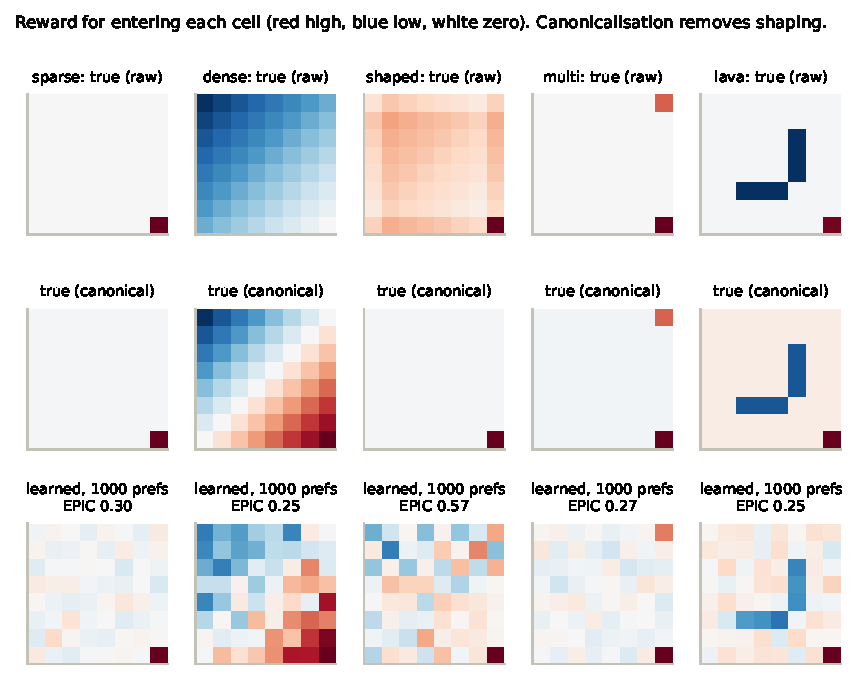
\includegraphics[width=0.82\linewidth]{../figures/fig1_shapes.pdf}
\caption{Reward for entering each cell. Top: the raw ground truth. Middle: its EPIC-canonical form (the shaped reward becomes the sparse one).
Bottom: canonical rewards learned from 1000 preference pairs (seed 0).}
\label{fig:shapes}
\end{figure}

\section{Results}
\subsection{How much feedback until recovery?}\label{sec:recovery}
Figure~\ref{fig:recovery} shows regret and EPIC against $N$. From preferences, $N^*$ was
\nstarprefssparse{} (sparse), \nstarprefsdense{} (dense), \nstarprefsshaped{} (shaped), \nstarprefsmulti{} (multi) and \nstarprefslava{} (lava).
From demonstrations it was \nstardemossparse, \nstardemosdense, \nstardemosshaped, \nstardemosmulti{} and \nstardemoslava.
\textbf{H1 is \Hone}: the sparse/dense ratio is \ratiosparsedense$\times$ and the lava/dense ratio \ratiolavadense$\times$.
In this setting, a sparse goal is easy to recover from comparisons. Our reading, untested: the compared trajectories are often near-optimal,
preferred ones end at the goal, and that alone is enough for a greedy policy. The uninformed controls (a random reward) score regret between \randregretlava{} and \randregretdense.

Two patterns we did not predict. \emph{First}, preference-based regret is not monotone in $N$ for dense
(\regprefsdensethirty, \regprefsdensehundred, \regprefsdensethreehundred, \regprefsdensethousand{} at $N=30,100,300,1000$) and shaped
(\regprefsshapedthirty, \regprefsshapedhundred, \regprefsshapedthreehundred, \regprefsshapedthousand). More preferences temporarily made the
policy worse. The optimizer is not the cause: 300 and 3000 L-BFGS iterations give identical fits. An exploratory check on the tuning seeds
also ruled out the action term $w(s,a)$: removing it does not remove the bump. We leave the mechanism open.
\emph{Second}, regret saturates long before the reward is identified. EPIC keeps falling up to $N=1000$, where it is still
\epicprefssparse--\epicprefsshaped{} from preferences, while regret has been near zero for many $N$. For shaped demonstrations,
EPIC barely moves (\epicdemosshaped{} at $N=1000$) even though regret reaches zero by $N=\nstardemosshaped$.

\begin{figure}[!htbp]\centering
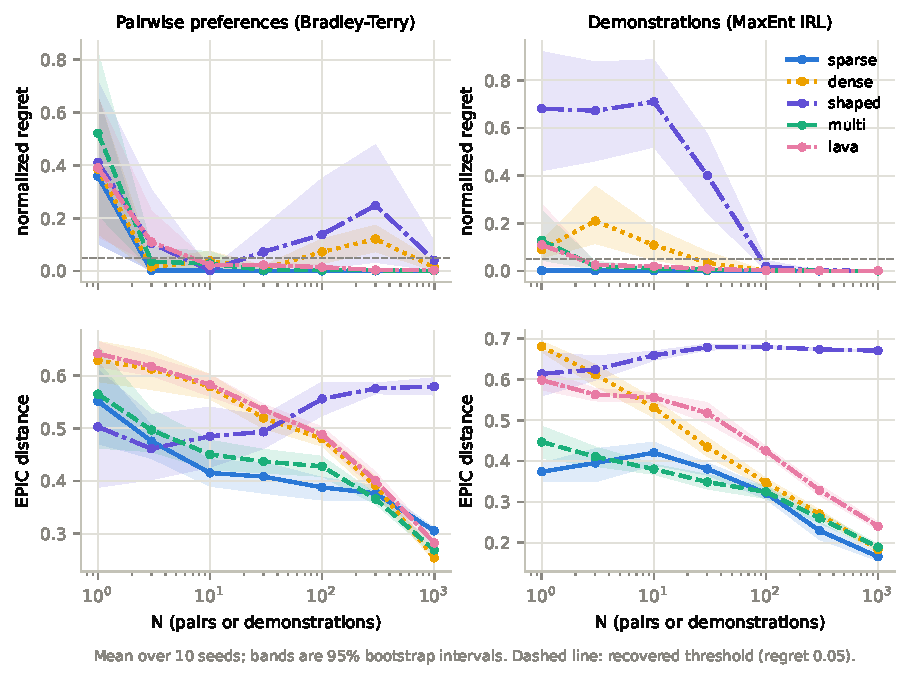
\includegraphics[width=0.88\linewidth]{../figures/fig2_recovery.pdf}
\caption{Normalized regret (top) and EPIC distance (bottom) against the amount of feedback. Mean over 10 seeds with 95\% bootstrap bands.}
\label{fig:recovery}
\end{figure}

\subsection{Which distance predicts regret?}\label{sec:metric}
Across all main runs, EPIC's Spearman correlation with regret is \rhoepicall{} against \rhopearsonall{} for raw Pearson
(difference \rhodiffall, 95\% CI [\rhodiffloall, \rhodiffhiall]); see Fig.~\ref{fig:metric}. \textbf{H2 is \Htwo.} The gap is concentrated where theory says it should be.
On the shaped reward, raw Pearson is almost uninformative ($\rho=\rhopearsonshaped$) while EPIC is not ($\rho=\rhoepicshaped$; difference
\rhodiffshaped{} [\rhodiffloshaped, \rhodiffhishaped]). Raw correlation is dominated by the shaping term, which does not affect the optimal policy.
For the other shapes the two metrics are within a few hundredths of each other. Correlations are weakest for dense
($\rho\approx\rhoepicdense$), because regret there is small and noisy at every $N$.

\begin{figure}[!htbp]\centering
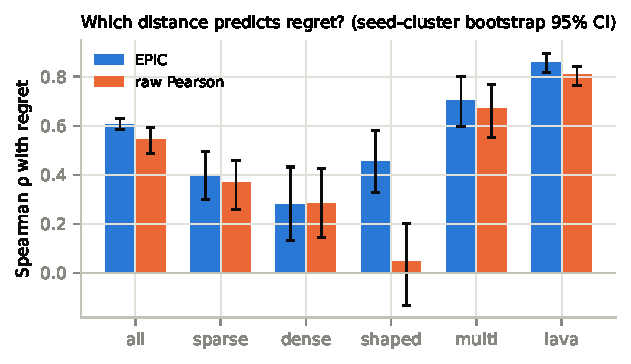
\includegraphics[width=0.62\linewidth]{../figures/fig3_metric.pdf}
\caption{Spearman correlation between each reward distance and normalized regret (seed-cluster bootstrap 95\% CI).}
\label{fig:metric}
\end{figure}

\subsection{When the labeler or the optimizer misbehaves}\label{sec:misspec}
\paragraph{Myopic labeler.} When the labeler discounts by 0.8 but the model assumes 0.95 (Fig.~\ref{fig:ablations}, left), regret at $N=1000$ is
\myopicsparse{} (sparse), \myopicdense{} (dense), \myopicshaped{} (shaped), \myopicmulti{} (multi) and \myopiclava{} (lava). With the
correct labeler it is at most \standardshaped. \textbf{H3 is \Hthree{} as stated}. The worst shapes are lava and shaped, not sparse
and lava. And regret is not flat in $N$: for every shape it is lowest around $N=10$ (sparse \regmyopicsparseten, lava \regmyopiclavaten)
and then rises (lava \regmyopiclavathousand{} at $N=1000$). One reading, which we did not test: with little data the $\ell_2$ prior dominates the bias, and with more data
the model fits the wrong discount confidently. Either way, in this setting more biased feedback was worse than less.

\paragraph{Labeler rationality.} Lower $\beta$ hurts the shaped reward far more than the others. At $N=300$, shaped regret is \regbetashapedthreehundredlow{}
at $\beta=0.3$, against \regbetadensethreehundredlow{} for dense and \regbetasparsethreehundredlow{} for sparse (Fig.~\ref{fig:ablations}, right).

\paragraph{Overoptimization.} Following \citet{gao2022scaling}, we optimize a learned proxy with a soft-optimal policy at increasing inverse
temperature $\lambda$ and score it on the true reward (Fig.~\ref{fig:overopt}). The true return rises and then plateaus, and in most cells it never turns down.
The exceptions are the $N=300$ proxies for dense and shaped, which peak and then lose \oodropdensec{} and \oodropshapedc{} of normalized return.
Those proxies also plateau below the ones learned from fewer pairs, which matches the mid-$N$ regret bump in \S\ref{sec:recovery}.
In this tabular setting, overoptimization is mild.

\begin{figure}[!htbp]\centering
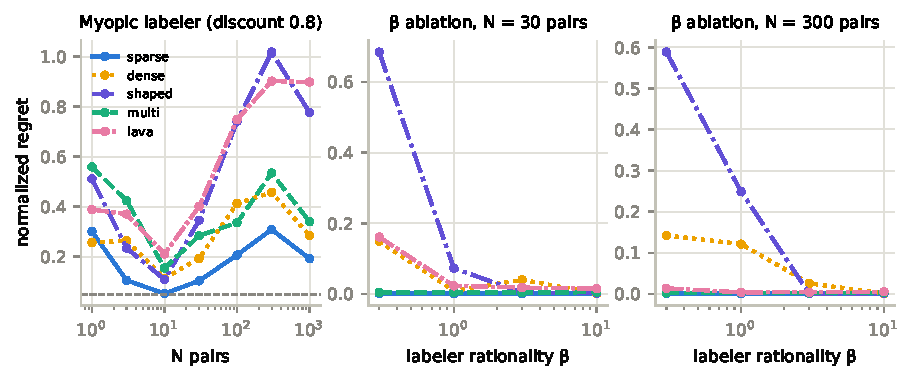
\includegraphics[width=\linewidth]{../figures/fig4_ablations.pdf}
\caption{Left: a myopic labeler (discount 0.8). Middle and right: labeler rationality $\beta$ at $N=30$ and $N=300$ pairs.}
\label{fig:ablations}
\end{figure}
\begin{figure}[!htbp]\centering
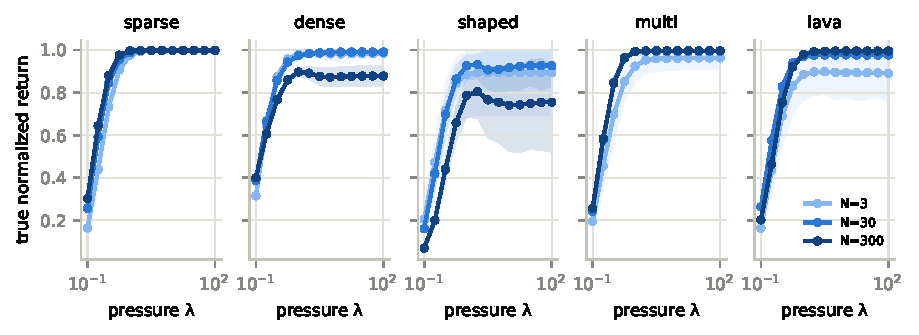
\includegraphics[width=\linewidth]{../figures/fig5_overopt.pdf}
\caption{True normalized return of the soft-optimal policy for a learned proxy, against optimization pressure $\lambda$.}
\label{fig:overopt}
\end{figure}

\subsection{Does shaping speed up learning?}\label{sec:shaping}
As a check on the \emph{use} of shaped rewards, tabular Q-learning (learning rate 0.1, $\epsilon=0.1$, 50-step episodes) was trained on the
sparse, dense or shaped reward and always scored on the sparse task (Fig.~\ref{fig:shaping}). The shaped reward cuts regret fastest in
the first few hundred episodes. Dense is slowest early. On the
pre-registered criterion (episodes until regret $\le0.05$), \qsolveddense/10 dense, \qsolvedshaped/10 shaped and only \qsolvedsparse/10 sparse seeds
crossed the threshold within 3000 episodes (median \qmediandense, \qmedianshaped{} and \qmediansparse{} episodes among those that did). Sparse
training plateaus at a regret of \qfinalsparse, just above the line; we did not diagnose why.

\begin{figure}[!htbp]\centering
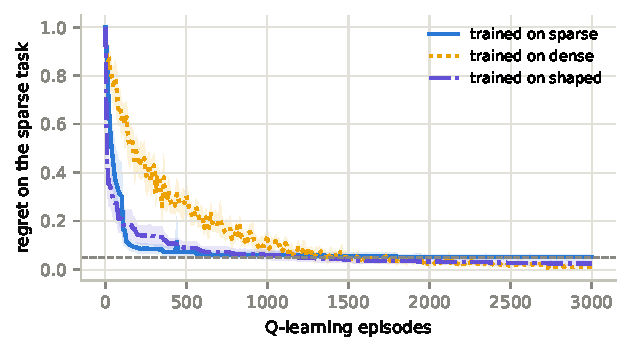
\includegraphics[width=0.62\linewidth]{../figures/fig6_shaping.pdf}
\caption{Regret on the sparse task during Q-learning on each training reward (10 seeds, 95\% bands).}
\label{fig:shaping}
\end{figure}

\section{Related work}
Preference-based reward learning goes back to paired-comparison models \citep{bradley1952rank} and was popularized for deep RL by
\citet{christiano2017deep}. \citet{knox2022models} question the return-based (Boltzmann) labeler that we also assume. Maximum-entropy
IRL \citep{ziebart2008maxent} is our demonstration learner. Potential shaping preserves optimal policies \citep{ng1999shaping}, and feedback
identifies rewards only up to such transformations \citep{skalse2023invariance}. EPIC \citep{gleave2021epic} and its dynamics-aware
successor DARD \citep{wulfe2022dard} compare rewards modulo shaping. \citet{skalse2023misspec} analyse how IRL degrades under a
misspecified behaviour model, which is the theory behind our myopic-labeler ablation. \citet{gao2022scaling} measure proxy overoptimization in language
models; Fig.~\ref{fig:overopt} is a tabular analogue.

\section{Limitations}
This is one small gridworld with simulated labelers, and the results should not be read as claims about reward learning in general. The
compared trajectories come from a generous $\epsilon$-greedy mixture around the optimal policy; uninformed sampling would make every shape
harder. The reward model is well specified (except under the myopic ablation), so we test identifiability, not misspecification of the model class.
EPIC over the uniform product space counts state--action pairs that no feedback constrains, so its floor stays above zero. A dynamics-aware
distance \citep{wulfe2022dard} might track regret better. Regret saturates quickly in gridworlds, so $N^*$ falls on the first few grid points
for most shapes; a 16$\times$16 check is deferred. The non-monotone regret curves are reported, not explained.

\paragraph{Invented parameters.} The grid size and layout, slip probability, $\gamma$, $H$, goal, lava and multi-goal values, step cost, the
unit-std rescaling, $\beta$, the $\epsilon$-mixture, the demonstrator's temperature, the myopic discount 0.8, the $\ell_2$ weight and the 0.05 threshold
were all chosen by us, not measured.

\paragraph{Reproducibility.} \texttt{uv run python -m rewardshapes.run\_all} regenerates every run, figure and number in this paper
(the environment is pinned in \texttt{uv.lock}). All raw runs are included.


\bibliographystyle{plainnat}
\bibliography{refs}
\end{document}
